% 方阵和同形矩阵的标量读数：行列式、迹与元素内积。
\section{行列式、迹与元素内积}
\label{sec:ls-matrix-scalar-readouts}

矩阵运算可以产生另一张数表，也可以产生一个标量。行列式衡量方阵作用下有向体积的缩放；迹累计主对角元素；Frobenius内积比较同形矩阵的全部对应元素。它们回答的问题不同，不能只凭其中一个数恢复原矩阵。

\subsection{行列式的定义与计算}
\phantomsection
\label{sec:ls-exterior-determinants}
\label{sec:linear-algebra-scalar-readouts}

一张方阵把单位正方形变成平行四边形、把单位立方体变成平行多面体时，面积或体积放大多少倍？平行四边形的面积不能由两条边的长度直接算出，它还取决于两个向量的相对方向；若再记录定向，交换两个向量的次序会使有向面积变号。下面先建立记录有向体积的外积，再由它得到行列式和它的计算公式。

\paragraph{外积}
对$\mathbb R^d$中的$k$个向量$\bm v_1,\ldots,\bm v_k$，它们的\term{外积}（exterior product，又称\term{楔积}wedge product）$\bm v_1\wedge\cdots\wedge\bm v_k$按两条规则计算。
\begin{itemize}
 \item 多线性：对每个因子分别保持线性组合，即把某个$\bm v_i$换成$a\bm u+b\bm w$时，整个楔积等于$a(\cdots\wedge\bm u\wedge\cdots)+b(\cdots\wedge\bm w\wedge\cdots)$，其余因子不动。
 \item 交替性：交换相邻两个因子，楔积变号，
 \[
  \cdots\wedge\bm v_i\wedge\bm v_j\wedge\cdots
  =-\cdots\wedge\bm v_j\wedge\bm v_i\wedge\cdots.
 \]
\end{itemize}

两条规则先给出两个推论。第一，含有两个相同因子的楔积为零：两个相同因子相邻时，交换它们不改变楔积，却使它变号，所以它等于自身的相反数，只能为零；两个相同因子不相邻时，先用相邻交换把它们移到一起，只改变符号，结论不变。第二，若某个因子是其余因子的线性组合，把这个因子按组合代入并由多线性展开，每一项都含有两个相同因子，所以整个楔积为零。

由此可以确定楔积的一般形状。

设$v_{j,i}$是$\bm v_j$的第$i$个坐标，把每个$\bm v_j=\sum_i v_{j,i}\bm e_i$代入并展开，含重复下标的项为零；其余各项按交替性把下标排成递增次序，只改变符号。所以每个楔积都是基楔积$\bm e_{i_1}\wedge\cdots\wedge\bm e_{i_k}$（$i_1<\cdots<i_k$）的线性组合，这样的基楔积共有$\binom{d}{k}$个。$k>d$时，每一项都必然含有重复下标，所以楔积恒为零。

对$\{1,\ldots,k\}$上的一般排列$\pi$，可以反复交换相邻的两个因子，把$\bm v_{\pi(1)}\wedge\cdots\wedge\bm v_{\pi(k)}$排回$\bm v_1\wedge\cdots\wedge\bm v_k$。记$N(\pi)$为$\pi$的逆序对数，即满足$i<j$而$\pi(i)>\pi(j)$的索引对数。每次交换一对相邻且次序颠倒的因子，逆序对数恰好减少$1$，所以恰好经过$N(\pi)$次交换就排好，每次交换变号一次，得到
\[
 \begin{gathered}
\bm v_{\pi(1)}\wedge\cdots\wedge\bm v_{\pi(k)}
 =\operatorname{sgn}(\pi)\,\bm v_1\wedge\cdots\wedge\bm v_k\\
\operatorname{sgn}(\pi)=(-1)^{N(\pi)}.
 \end{gathered}
\]

\paragraph{有向面积与有向体积}
在$\mathbb R^2$中按两条规则展开，
\[
 \bm u\wedge\bm v
 =(u_1\bm e_1+u_2\bm e_2)\wedge(v_1\bm e_1+v_2\bm e_2)
 =(u_1v_2-u_2v_1)\,\bm e_1\wedge\bm e_2,
\]
其中用到$\bm e_1\wedge\bm e_1=\bm e_2\wedge\bm e_2=0$与$\bm e_2\wedge\bm e_1=-\bm e_1\wedge\bm e_2$。系数$u_1v_2-u_2v_1$是$\bm u,\bm v$张成的平行四边形的有向面积：绝对值是面积，符号是定向。

下面用三组向量观察有向面积的数值与符号。
\begin{example}[平面上的有向面积]
\label{ex:ls-oriented-area}
给定：三组有序向量对：$\bm u=(1,0)^\top$与$\bm v=(1,1)^\top$；交换次序后的$\bm v$与$\bm u$；共线的$(1,1)^\top$与$(2,2)^\top$。
计算：按系数公式$u_1v_2-u_2v_1$，三组依次得到
\[
 \begin{gathered}
1\cdot1-0\cdot1=1\\
1\cdot0-1\cdot1=-1\\
1\cdot2-1\cdot2=0.
 \end{gathered}
\]
结论：第一组张成面积为$1$的平行四边形；交换次序后面积不变而定向翻转，所以符号变负；共线的两个向量张成的平行四边形退化成线段，有向面积为$0$。
\end{example}
由上面的计数，$\mathbb R^3$中三个向量的楔积只是基楔积$\bm e_1\wedge\bm e_2\wedge\bm e_3$的倍数。这个系数的绝对值是三个向量张成的平行六面体的体积，带符号时称为\term{有向体积}。

\paragraph{行列式的定义}
在$\mathbb R^d$中取$d$个向量，最高阶楔积只剩一个基楔积$\bm e_1\wedge\cdots\wedge\bm e_d$。对$d$阶方阵$\bm A$，把它的各列$\bm A\bm e_1,\ldots,\bm A\bm e_d$作楔积，
\[
 \bm A\bm e_1\wedge\cdots\wedge\bm A\bm e_d
 =(\det\bm A)\,\bm e_1\wedge\cdots\wedge\bm e_d,
\]
标量$\det\bm A$称为\term{行列式}（determinant）。它是$\bm A$把单位立方体变成平行多面体时的有向体积倍数，绝对值为体积比，符号表示定向是否翻转。图~\ref{fig:ls-determinant-oriented-volume}在平面上画出这一缩放。
\begin{figure*}[htbp]
  \centering
  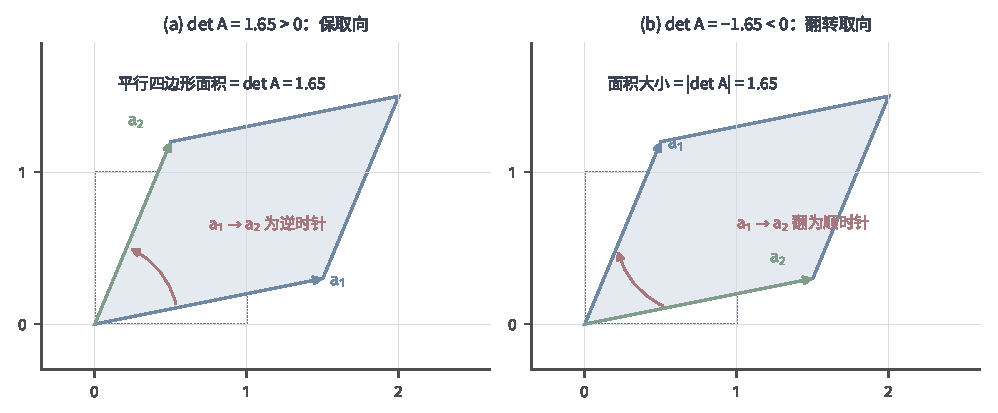
\includegraphics[width=169mm]{figures/00-shared/mathematical-preliminaries-upper/02-linear-spaces/matplotlib/ls-determinant-oriented-volume/ls-determinant-oriented-volume.pdf}
  \caption{行列式作为有向体积的缩放。左：单位正方形由$\bm e_1=(1,0)$、$\bm e_2=(0,1)$张成，面积为$1$。中：$\bm A=\bigl(\begin{smallmatrix}2&0.5\\0&1.5\end{smallmatrix}\bigr)$把它映成由$\bm A\bm e_1=(2,0)$、$\bm A\bm e_2=(0.5,1.5)$张成的平行四边形，有向面积为$2\cdot1.5-0.5\cdot0=3=\det\bm A>0$（保定向）。右：$\bm A$把$\bm e_1$反射到$(-2,0)$，有向面积为$-3$（反定向）。向量与数值均为解析教学例。}
  \label{fig:ls-determinant-oriented-volume}
\end{figure*}

\paragraph{排列展开}
把$\bm A\bm e_j=\sum_i a_{i,j}\bm e_i$代入楔积并展开。若第$j$个因子选出$\bm e_{\tau(j)}$，得到的项为$\bigl(\prod_ja_{\tau(j),j}\bigr)\,\bm e_{\tau(1)}\wedge\cdots\wedge\bm e_{\tau(d)}$。下标有重复的项为零；留下的项中$\tau$是$\{1,\ldots,d\}$的一个排列，而$\bm e_{\tau(1)}\wedge\cdots\wedge\bm e_{\tau(d)}=\operatorname{sgn}(\tau)\,\bm e_1\wedge\cdots\wedge\bm e_d$。所以
\[
 \det\bm A=\sum_{\tau}\operatorname{sgn}(\tau)\prod_{j=1}^d a_{\tau(j),j},
\]
求和遍历全部排列。习惯上按行书写：记$\pi=\tau^{-1}$，把乘积按行号重排，得到$\prod_ia_{i,\pi(i)}$。$\tau$的逆序对$(i,j)$与$\pi$的逆序对$(\tau(j),\tau(i))$一一对应，所以$\operatorname{sgn}(\pi)=\operatorname{sgn}(\tau)$。于是得到计算公式
\[
 \det\bm A
 =\sum_{\pi\in S_d}\operatorname{sgn}(\pi)
   \prod_{i=1}^d a_{i,\pi(i)},
\]
其中$S_d$是$\{1,\ldots,d\}$到自身的全部双射，每个$\pi$规定第$i$行选取第$\pi(i)$列。计算步骤是：对每个排列，从每行各取一个元素、各列恰好取一次，把取出的$d$个数相乘，再按逆序对数的奇偶加上正负号求和。

二阶时只有两个排列：恒等排列没有逆序对，取正号；交换$1,2$的排列有一个逆序对，取负号。于是
\[
 \det\begin{pmatrix}a&b\\c&d\end{pmatrix}=ad-bc,
\]
例如$\det\left(\begin{smallmatrix}1&2\\3&4\end{smallmatrix}\right)=1\cdot4-2\cdot3=-2$。

三阶时有六个排列。恒等排列与两个循环排列$(\pi(1),\pi(2),\pi(3))=(2,3,1)$、$(3,1,2)$的逆序对数为$0$或$2$，取正号；只交换两个位置的三个排列$(1,3,2)$、$(2,1,3)$、$(3,2,1)$的逆序对数为$1$或$3$，取负号。于是
\[
 \begin{aligned}
 \det\bm A={}&a_{1,1}a_{2,2}a_{3,3}+a_{1,2}a_{2,3}a_{3,1}+a_{1,3}a_{2,1}a_{3,2}\\
 &-a_{1,1}a_{2,3}a_{3,2}-a_{1,2}a_{2,1}a_{3,3}-a_{1,3}a_{2,2}a_{3,1}.
 \end{aligned}
\]
下面用这个公式计算一个具体的三阶行列式。
\begin{example}[三阶行列式的排列展开]
\label{ex:ls-det-three-by-three}
给定：$\bm A=\left(\begin{smallmatrix}2&0&1\\1&3&0\\0&1&1\end{smallmatrix}\right)$。
计算：按上式的六项次序代入，
\[
 \begin{aligned}
 \det\bm A&=2\cdot3\cdot1+0\cdot0\cdot0+1\cdot1\cdot1-2\cdot0\cdot1-0\cdot1\cdot1-1\cdot3\cdot0\\
 &=6+0+1-0-0-0=7.
 \end{aligned}
\]
结论：$\det\bm A=7$。六项中只有两项非零，其余四项都含有零元素。
\end{example}

行列式因而是矩阵元素的多项式。上面的推导只说明：若楔积满足两条规则，行列式只能是这个和。反过来可以直接验证，排列展开式作为各列的函数确实对每列线性、交换两列时变号（交换两列相当于把每个$\pi$复合上一次对换，逆序对数的奇偶随之改变），并且在单位矩阵处等于$1$。所以两条规则彼此相容，行列式由它们和$\det\bm I_d=1$唯一确定。高阶时排列有$d!$个，实际计算通常利用下面的性质和消元。



\subsection{行列式的性质与可逆性}
\label{sec:ls-determinant-properties}
\phantomsection
\label{sec:prelim-determinants}

行列式由楔积的两条规则定义，下面前两条性质就是这两条规则在列上的表述，其余性质由它们推出。

设$\bm A,\bm B$为$d$阶方阵。

\paragraph{对列的多线性}
\[
 \det\begin{bmatrix}\cdots&a\bm u+b\bm w&\cdots\end{bmatrix}
 =a\det\begin{bmatrix}\cdots&\bm u&\cdots\end{bmatrix}
 +b\det\begin{bmatrix}\cdots&\bm w&\cdots\end{bmatrix},
\]
其中三个矩阵只在同一列不同，其余各列相同。$\det\bm A$是各列楔积的系数，所以这正是楔积对每个因子保持线性组合的直接翻译。

\paragraph{交替性}
交换两列，行列式变号；两列相同，行列式为零。前者来自楔积交换两个因子时变号（不相邻的两个因子可以经奇数次相邻交换互换位置）；后者是因为交换两个相同的列不改变矩阵，行列式却要变号，只能为零。

两条合起来又得到两个常用推论。把某列的倍数加到另一列上，行列式不变：按多线性拆开，多出的一项含两列相同，为零。某一列是其余各列的线性组合时，行列式为零：把这一列按组合展开，每一项都含两列相同。例如$\det\left(\begin{smallmatrix}1&2\\2&4\end{smallmatrix}\right)=4-4=0$，第二列是第一列的$2$倍。

\paragraph{转置不变}
\[
 \det(\bm A^\top)=\det\bm A.
\]
在排列展开中，把每一项的乘积按列号重排，得$\prod_ia_{i,\pi(i)}=\prod_ja_{\pi^{-1}(j),j}$；排列展开的推导已经说明$\operatorname{sgn}(\pi^{-1})=\operatorname{sgn}(\pi)$。$\pi$遍历$S_d$时，$\sigma=\pi^{-1}$也遍历$S_d$，所以
\[
 \det\bm A=\sum_{\sigma\in S_d}\operatorname{sgn}(\sigma)\prod_{j=1}^da_{\sigma(j),j}
 =\sum_{\sigma\in S_d}\operatorname{sgn}(\sigma)\prod_{j=1}^d(\bm A^\top)_{j,\sigma(j)}
 =\det(\bm A^\top).
\]
于是对列成立的多线性与交替性，对行同样成立。

\paragraph{行变换与可逆性}
行上的多线性和交替性给出三条计算规则：交换两行使行列式变号；某行乘以非零数$c$使行列式乘以$c$；某行加上另一行的倍数不改变行列式。第三条是因为按该行展开后，多出的矩阵有两行相同，其行列式为零。

用这些规则配合消元，可以把方阵化为上三角矩阵，再取对角元素的乘积并补偿换行及倍乘的影响。例如
\[
 \det\begin{pmatrix}0&1&2\\1&2&1\\2&7&4\end{pmatrix}
 =-\det\begin{pmatrix}1&2&1\\0&1&2\\0&3&2\end{pmatrix}
 =-\det\begin{pmatrix}1&2&1\\0&1&2\\0&0&-4\end{pmatrix}=4.
\]
第一步交换前两行，并从第三行减去第一行的两倍；第二步再从第三行减去第二行的三倍。交换行使符号改变，两次加倍数不改变行列式。

这也把行列式与求逆联系起来。消元中的每一步都可逆，而且只使行列式乘以一个非零数。

若每列都找到主元，阶梯形是对角元非零的上三角矩阵，故行列式非零，并可继续化为单位矩阵求逆。

若某列找不到主元，方阵的阶梯形至少有一行全零，行列式为零，也无法化为单位矩阵。因此方阵可逆当且仅当其行列式非零。

\paragraph{数乘与加法}
\[
\begin{gathered}
\det(c\bm A)=c^d\det\bm A\\
\det(\bm A+\bm B)\neq\det\bm A+\det\bm B\ (\text{一般}).
\end{gathered}
\]
数乘把$d$列各乘以$c$，由对每列的线性提出$d$个$c$。行列式只对每一列分别线性，对整个矩阵却不是线性的，下面是一个反例。
\begin{example}[反例：行列式不保持加法]
\label{ex:ls-det-not-additive}
给定：$\bm A=\bm B=\bm I_2$。
计算：$\det\bm A+\det\bm B=1+1=2$，而由第一式，$\det(\bm A+\bm B)=\det(2\bm I_2)=2^2\det\bm I_2=4$。
结论：$\det(\bm A+\bm B)\neq\det\bm A+\det\bm B$。
\end{example}

\paragraph{乘法性}
\[
 \det(\bm A\bm B)=\det\bm A\,\det\bm B.
\]
接连作用两次时，体积缩放倍数应当相乘。排列展开的推导只用到楔积的两条规则，所以把$\bm e_1,\ldots,\bm e_d$换成任意向量$\bm w_1,\ldots,\bm w_d$，同样有$\bigwedge_j\bigl(\sum_ib_{i,j}\bm w_i\bigr)=(\det\bm B)\,\bm w_1\wedge\cdots\wedge\bm w_d$。由$(\bm A\bm B)\bm e_j=\bm A(\bm B\bm e_j)=\sum_i b_{i,j}\bm A\bm e_i$，取$\bm w_i=\bm A\bm e_i$，得到
\[
 (\bm A\bm B)\bm e_1\wedge\cdots\wedge(\bm A\bm B)\bm e_d
 =(\det\bm B)\,\bm A\bm e_1\wedge\cdots\wedge\bm A\bm e_d
 =(\det\bm A)(\det\bm B)\,\bm e_1\wedge\cdots\wedge\bm e_d.
\]
尽管矩阵乘法不可交换，$\det(\bm A\bm B)=\det(\bm B\bm A)$总成立，因为两边都等于$\det\bm A\,\det\bm B$。

\paragraph{三角矩阵的行列式}
\[
 \det\bm A=a_{1,1}a_{2,2}\cdots a_{d,d}\qquad(\bm A\text{为上三角或下三角矩阵}).
\]
设$\bm A$为上三角矩阵。排列$\pi$不是恒等排列时，必有某行$i$满足$\pi(i)<i$（因为$\sum_i(\pi(i)-i)=0$而各项不全为零），这一行选到主对角线下方的零元素，所以这一项为零；排列展开中只剩恒等排列一项。下三角时同理。例如$\det\left(\begin{smallmatrix}1&2&3\\0&4&5\\0&0&6\end{smallmatrix}\right)=1\cdot4\cdot6=24$；特别地，$\det\operatorname{diag}(d_1,\ldots,d_d)=d_1\cdots d_d$，$\det\bm I=1$。与乘法性合起来，两个上三角矩阵乘积的行列式就是两者全部对角元之积，这与三角矩阵乘积的对角元逐个相乘一致。

\paragraph{按行（列）展开}
对$d\geq2$，删除第$i$行、第$j$列得到的$(d-1)$阶子矩阵记为$\bm A^{(i,j)}$，定义\term{代数余子式}（cofactor）
\[
 C_{i,j}=(-1)^{i+j}\det\bm A^{(i,j)}.
\]
则对任一行$i$与任一列$j$，
\[
 \det\bm A=\sum_{j=1}^d a_{i,j}C_{i,j}=\sum_{i=1}^d a_{i,j}C_{i,j}.
\]
把排列展开按第$i$行选取的列分类，选第$j$列的各项之和正是$a_{i,j}C_{i,j}$；按列同理。下面沿第一行展开示例~\ref{ex:ls-det-three-by-three}中的矩阵，与排列展开的结果对照。
\begin{example}[沿第一行展开三阶行列式]
\label{ex:ls-det-cofactor-expansion}
给定：$\bm A=\left(\begin{smallmatrix}2&0&1\\1&3&0\\0&1&1\end{smallmatrix}\right)$。
计算：第一行元素为$2,0,1$，对应代数余子式的符号依次为$+,-,+$，
\[
 \begin{aligned}
 \det\bm A
 &=2\cdot\det\begin{pmatrix}3&0\\1&1\end{pmatrix}
 -0\cdot\det\begin{pmatrix}1&0\\0&1\end{pmatrix}
 +1\cdot\det\begin{pmatrix}1&3\\0&1\end{pmatrix}\\
 &=2\cdot3-0\cdot1+1\cdot1=7.
 \end{aligned}
\]
结论：结果与示例~\ref{ex:ls-det-three-by-three}的排列展开一致。
\end{example}

\paragraph{古典伴随恒等式}
把全部代数余子式排成矩阵$\bm C$，其转置称为\term{古典伴随}（classical adjugate）$\operatorname{adj}(\bm A)=\bm C^\top$。
\begin{theorem}[古典伴随恒等式]
\label{thm:ls-adjugate-identity}
对任意$d$阶方阵$\bm A$，
\[
 \bm A\,\operatorname{adj}(\bm A)
 =\operatorname{adj}(\bm A)\,\bm A
 =(\det\bm A)\,\bm I_d.
\]
\end{theorem}
\begin{proof}
乘积$\bm A\bm C^\top$的$(i,k)$元素为$\sum_j a_{i,j}C_{k,j}$。当$i=k$时，这正是沿第$i$行展开的$\det\bm A$。当$i\neq k$时，$C_{k,j}$不涉及第$k$行的元素，所以这个和是把第$k$行换成第$i$行后的矩阵沿第$k$行的展开；新矩阵有两行相同，行列式为零。于是$\bm A\bm C^\top=(\det\bm A)\bm I_d$。按列展开同样得到$\bm C^\top\bm A=(\det\bm A)\bm I_d$。
\end{proof}
二阶时$\operatorname{adj}\left(\begin{smallmatrix}a&b\\c&d\end{smallmatrix}\right)=\left(\begin{smallmatrix}d&-b\\-c&a\end{smallmatrix}\right)$，恒等式两边除以$ad-bc$就是第~\ref{sec:prelim-inverse-matrices}节的二阶求逆公式。

古典伴随是由余子式得到的代数构造，与第~\ref{sec:ls-inner-product-spaces}节由内积配对定义的伴随不是同一个对象。高阶时展开余子式的代价是阶乘级的，所以恒等式主要作为证明工具：下面用它证明方阵的单侧逆即逆，第~\ref{sec:ls-determinant-invertibility}节用它给出可逆判据，第~\ref{sec:ls-characteristic-polynomial}节用它证明Cayley--Hamilton定理。

\paragraph{方阵的单侧逆即逆}
\phantomsection
\label{sec:ls-square-one-sided-inverse}
若$n$阶方阵满足$\bm B\bm A=\bm I_n$或$\bm A\bm B=\bm I_n$，则$\bm A$可逆且$\bm B=\bm A^{-1}$。

由乘法性，两种情形都有$\det\bm A\det\bm B=\det\bm I_n=1$，所以$\det\bm A\neq0$。令$\bm C=\operatorname{adj}(\bm A)/\det\bm A$，古典伴随恒等式给出$\bm A\bm C=\bm C\bm A=\bm I_n$，所以$\bm A$可逆，$\bm C=\bm A^{-1}$。若$\bm B\bm A=\bm I_n$，则$\bm B=\bm B(\bm A\bm C)=(\bm B\bm A)\bm C=\bm C$；若$\bm A\bm B=\bm I_n$，则$\bm B=(\bm C\bm A)\bm B=\bm C(\bm A\bm B)=\bm C$。所以检查方阵的逆只需验证一侧的乘积。对矩形矩阵，左逆与右逆则可以只存在一个，也可以不唯一（示例~\ref{ex:ls-left-inverse-not-unique}）。

\subsection{迹}
\label{sec:prelim-matrix-trace}

$n$阶方阵的\term{迹}（trace）是主对角元素之和：
\[
 \operatorname{tr}(\bm A)=\sum_{i=1}^n A_{i,i}.
\]
例如$\operatorname{tr}\left(\begin{smallmatrix}1&2\\3&4\end{smallmatrix}\right)=1+4=5$，而这个矩阵全部元素之和是$10$。迹只对方阵定义，只累加对角元。


\subsubsection{迹的性质}
\phantomsection
\label{sec:ls-matrix-contractions}

\paragraph{线性}
\[
 \operatorname{tr}(a\bm A+b\bm B)=a\operatorname{tr}(\bm A)+b\operatorname{tr}(\bm B),
\]
这是有限和的线性。

\paragraph{转置不变}
\[
 \operatorname{tr}(\bm A^\top)=\operatorname{tr}(\bm A),
\]
因为转置不改变对角元。

\paragraph{循环性}
对$\bm A\in\mathbb R^{m\times n}$、$\bm B\in\mathbb R^{n\times m}$，
\begin{equation}
 \operatorname{tr}(\bm A\bm B)
 =\sum_{i=1}^m\sum_{j=1}^n A_{i,j}B_{j,i}
 =\operatorname{tr}(\bm B\bm A).
 \label{eq:linear-algebra-trace-cyclic}
\end{equation}
两个双重和只是求和次序不同。$\bm A\bm B$与$\bm B\bm A$可以是不同阶的方阵，相等的是迹，不是矩阵本身，下面的例子说明这一点。
\begin{example}[不同阶乘积的迹相等]
\label{ex:ls-trace-cyclic-different-sizes}
给定：$\bm A=\left[\begin{smallmatrix}1&2&3\end{smallmatrix}\right]\in\mathbb R^{1\times3}$，$\bm B=(1,0,2)^\top\in\mathbb R^{3\times1}$。
计算：$\bm A\bm B=1\cdot1+2\cdot0+3\cdot2=7$是$1\times1$矩阵；
\[
 \bm B\bm A=\begin{bmatrix}1&2&3\\0&0&0\\2&4&6\end{bmatrix}
\]
是$3\times3$矩阵，对角元为$1,0,6$。
结论：$\operatorname{tr}(\bm A\bm B)=7=1+0+6=\operatorname{tr}(\bm B\bm A)$，而两个乘积的阶数不同。
\end{example}

三个因子时，循环性只允许把因子整体循环移动：
\[
 \operatorname{tr}(\bm A\bm B\bm C)=\operatorname{tr}(\bm B\bm C\bm A)=\operatorname{tr}(\bm C\bm A\bm B).
\]
第一个等号把$\bm A$与$\bm B\bm C$看作两个因子使用式~\eqref{eq:linear-algebra-trace-cyclic}，第二个等号把$\bm A\bm B$与$\bm C$看作两个因子。任意交换相邻因子则可能改变迹，下面是一个反例。
\begin{example}[反例：交换相邻因子会改变迹]
\label{ex:ls-trace-adjacent-swap}
给定：$\bm A=\left(\begin{smallmatrix}1&0\\0&0\end{smallmatrix}\right)$，$\bm B=\left(\begin{smallmatrix}0&0\\1&0\end{smallmatrix}\right)$，$\bm C=\left(\begin{smallmatrix}0&1\\0&0\end{smallmatrix}\right)$。
计算：$\bm A\bm B=\bm0$，所以$\bm A\bm B\bm C=\bm0$。另一方面$\bm A\bm C=\bm C$，所以
\[
 \bm A\bm C\bm B=\begin{pmatrix}0&1\\0&0\end{pmatrix}\begin{pmatrix}0&0\\1&0\end{pmatrix}=\begin{pmatrix}1&0\\0&0\end{pmatrix}.
\]
结论：$\operatorname{tr}(\bm A\bm B\bm C)=0$，而$\operatorname{tr}(\bm A\bm C\bm B)=1$；交换$\bm B$与$\bm C$的次序改变了迹。
\end{example}


\subsection{矩阵的元素内积}
\subsubsection{Frobenius内积}

把同形矩阵的$mn$个元素看作有限个坐标，照搬欧氏内积，就得到同形矩阵之间的\term{Frobenius内积}：对$\bm A,\bm B\in\mathbb R^{m\times n}$，
\[
 \langle\bm A,\bm B\rangle_{\mathrm F}=\sum_{i=1}^m\sum_{j=1}^na_{i,j}b_{i,j},
\]
即逐项相乘后全部相加，也就是$\bm A\odot\bm B$全部元素之和。下面沿用逐项乘积一例中的两个矩阵。
\begin{example}[Frobenius内积的计算]
\label{ex:ls-frobenius-inner-product}
给定：$\bm A=\left(\begin{smallmatrix}1&2\\3&4\end{smallmatrix}\right)$，$\bm B=\left(\begin{smallmatrix}0&1\\1&0\end{smallmatrix}\right)$。
计算：
\[
 \langle\bm A,\bm B\rangle_{\mathrm F}=1\cdot0+2\cdot1+3\cdot1+4\cdot0=5.
\]
结论：结果等于示例~\ref{ex:ls-hadamard-vs-matrix-product}中$\bm A\odot\bm B$的元素之和$0+2+3+0=5$。
\end{example}

\paragraph{Frobenius内积的迹表示}
\[
 \begin{gathered}
 \langle\bm A,\bm B\rangle_{\mathrm F}=\operatorname{tr}(\bm A^\top\bm B),\\
 \lVert\bm A\rVert_{\mathrm F}^2=\operatorname{tr}(\bm A^\top\bm A).
 \end{gathered}
\]
$\bm A^\top\bm B$的第$j$个对角元为$\sum_i A_{i,j}B_{i,j}$，再对$j$求和恰好遍历所有位置。反过来，计算$\operatorname{tr}(\bm A\bm B)$时也不必形成乘积：只需算$\sum_{i,j}A_{i,j}B_{j,i}$，代价为$mn$次乘法，而形成整个$\bm A\bm B$需要$m^2n$次。



\subsubsection{Frobenius范数}
\label{sec:ls-frobenius-norm}

矩阵的“大小”有两种口径。第一种把矩阵当作数表，由Frobenius内积给出Frobenius范数
\[
 \lVert\bm A\rVert_{\mathrm F}=\sqrt{\langle\bm A,\bm A\rangle_{\mathrm F}}=\left(\sum_{i,j}a_{i,j}^2\right)^{1/2}.
\]
例如$\lVert\left(\begin{smallmatrix}1&2\\3&4\end{smallmatrix}\right)\rVert_{\mathrm F}=\sqrt{1+4+9+16}=\sqrt{30}$。它就是把$mn$个元素排成一列以后的$2$范数，其范数性质将在第~\ref{sec:ls-normed-space-definition}节由Minkowski不等式统一验证。

Frobenius范数也可以按作用来读。由$\bm A\bm e_j=\bm A_{:,j}$，
\[
 \lVert\bm A\rVert_{\mathrm F}^2=\sum_j\lVert\bm A_{:,j}\rVert_2^2=\sum_j\lVert\bm A\bm e_j\rVert_2^2,
\]
它是全部标准坐标输入所产生的输出平方和，而不是某一个最坏输入的放大。

需要先分组再汇总时，还可以用混合范数，例如以行为组的$\lVert\bm A\rVert_{p,q}=(\sum_i\lVert\bm A_{i,:}\rVert_p^q)^{1/q}$：内层的$p$范数衡量每组的大小，外层的$q$范数汇总各组。
